\documentclass[pdftex,12pt,a4paper]{report}

\usepackage{amsmath}
\usepackage{amsfonts}
\usepackage{amssymb}

\usepackage[ngerman]{babel}
\usepackage[utf8]{inputenc}


\usepackage[pdftex]{graphicx}
\usepackage{listings}

% new commands
\newcommand{\HRule}{\rule{\linewidth}{0.5mm}}


\author{Nik\v{s}a Ra\v{s}i\'{c};Martin Weinberg}
\title{Proposal Projekt}

\begin{document}
\title{Projektproposal:}
\date{09.01.13}
\author{Nik\v{s}a Ra\v{s}i\'{c} \& Martin Weinberg}

\begin{titlepage}
\begin{center}
% Upper part of the page
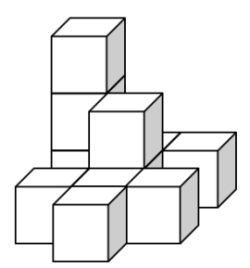
\includegraphics[width=0.4\textwidth]{./wuerfel}\\[1cm]    

\textsc{\LARGE Projektproposal}\\[1.5cm]

\textsc{\Large Creative Coding WS 12/13 }\\[0.5cm]


% Title
\HRule \\[0.4cm]
{ \huge \bfseries Emitting Cubes}\\[0.4cm]

\HRule \\[1.5cm]

% Author and supervisor
\begin{minipage}{0.4\textwidth}
\begin{flushleft} \large
\emph{Author:}\\
Nik\v{s}a Ra\v{s}i\'{c}  \&  \\ Martin Weinberg
\end{flushleft}
\end{minipage}
\begin{minipage}{0.4\textwidth}
\begin{flushright} \large
\emph{Supervisor:} \\ 
M. Sc.Alexander Neumann 
\end{flushright}
\end{minipage}

\vfill

% Bottom of the page
{\large \today}

\end{center}

\end{titlepage}

\tableofcontents
\newpage

\chapter{Emitting Cubes }
\section{Inspiration und Idee}
\section{Intention}
\section{Aufbau und Techniken}



\chapter{Konzepte mit Emitting Cubes}
\section{''Snake-around-the-Edge''}
\subsection{Ausgangspunkt}
Oftmals kommt es zu folgender Situation:\\
Man muss zum Amt um irgendeine Belanglosigkeit zu klären.\\
Aber bevor man mit jemandem dort sprechen kann um ihm zu erklären, dass man kein illegaler Einwanderer ist, sondern einfach jemand einen Accent in seinem Namen vergessen hat muss man warten.
Diese Wartezeit wird oft damti verbracht, Bücher zu lesen oder mit seinem Handy herumzuspielen - alleine...\\
...und hier kommen die Emitting Cubes ins Spiel!

\subsection{Die Idee und der Aufbau}
Um die Wartezeit an solchen Orten ein wenig zu verkürzen und zugleich, um für Gesellschaft bei der Tätigkeit des Herumsitzens zu schaffen, wurde ein Spiel nur für die Cubes entwickelt:\\
\\
\textbf{''Snake-around-the-Edge''}
\\\\
Ein Emitting Cube wird in der Mitte solcher Wartebereiche aufgehängt und von einem Beamer mit Spiegelsystem oder zwei Beamern von allen Seiten mittels Projection-Mapping angestrahlt.
Weiterhin existieren an mindestens sechs Plätzen kleine Tastaturen (es reichen hierbei Richtungs- und eine Start/Ende-Taste), die mit einem Stahlseil fest an dem jeweiligen Platz befestigt sind, um Diebstahl zu vermeiden.
Diese Tastaturen können per Funk mit dem Rechner, der den Beamer steuert, kommunizieren.

\subsection{Das Spiel}
Das Spielprinzip muss in einer solchen Umgebung natürlich einfach und jederzeit unterbrechbar sein.\\
Das Spielprinzip ist wie folgt:\\
\\
Man spielt eine Schlange, die Äpfel fressen muss. Sie bewegt sich automatisch in die Richtung weiter, die als letztes angewähklt wurde.
Es gibt auf dem Spielfeld eine bestimmte Anzahl Äpfel, die vom Rechner zufällig verteilt werden.
Wenn man einen Apfel frisst (sich darüber schlängelt) verschwindet der Apfel und irgendwo auf dem Spielfeld taucht ein neuer auf.
Außerdem wird die Schlange um ein bestimmtes Stück länger, wenn sie einen Apfel frisst.
Es gibt sonst nur zwei weitere Regeln: Die Schlange darf sich nicht selbst fressen und auch nicht eine Wand berühren.

\subsection{Umsetzung}
Das besondere an der Umsetzung mit dem Emitting Cube ist nun, dass sich das Spielfeld theoretisch über alle sechs Flächen des Würfels erstrecken kann.
Wenn eine Person das Spiel mit seinem Start-Button startet, wird es auf der ihm am nächsten gelegenen Fläche angezeigt.
Diese Fläche wird durch Triangulation mit mehreren Empfängern im Würfel bei der Kommunikation mit der Tastatur ermittelt.
Idealerweise hat eine Tastatur aber auch noch eine eindeutige Farbe, mit der die aktive Fläche jeweils leicht eingefärbt wird.
Nun kann dieser erste Spieler auf seiner Fläche spielen.
Dabei hat er allerdings die Einschränkung, dass die Fläche von Wänden umgeben ist.\\
\\
Möchte nun ein anderer Spieler mitspielen drückt er auf seiner Tastatur die Start-Taste.
Falls die ermittelte nächste Fläche an der des bereits spielenden anliegt, wird diese Wand nun bei beiden Spielern entfernt und sie können über die Würfelseite hinaus miteinander spielen.
Sobald der ''Kopf'' der Schlange die Würfelkante passiert, hat also der neue Spieler die Kontrolle und umgekehrt.
Dabei ist beim Design des Spiels darauf zu achten, dass neue Äpfel auf einer jeweils anderen Seite als der, 
auf der die Schlange sich gerade befindet, erzeugt werden, um zu verhindern, dass ein Spieler die ganze Zeit auf seiner Seite bleiben kann.

\subsection{Mehrfachnutzen}
Natürlich soll der Würfel auch informieren.
Daher ist geplant, dass beliebige Inhalte - also vom Betreiber aus vorgebbar - 
auf den restlichen Würfelflächen angezeigt, oder über Spielflächen mit einer gewissen Transparenz herübergelegt werden können.
Damit wird es möglich, dass der Betreiber Werbung schaltet oder die aktuellen Wartenummern auf allen Flächen des Würfels sichtbar sind.

\section{Perspektivlosigkeit}
Die Würfel mti Kamerabildern aus verschiedeneen Perspektiven in die man sich reinfinden muss 

\end{document}






